%%%%%%%%%%%%%%%%%%%%%%%%%%%%%%%%%%%%%%%%%
% Short Sectioned Assignment
% LaTeX Template
% Version 1.0 (5/5/12)
%
% This template has been downloaded from:
% http://www.LaTeXTemplates.com
%
% Original author:
% Frits Wenneker (http://www.howtotex.com)
%
% License:
% CC BY-NC-SA 3.0 (http://creativecommons.org/licenses/by-nc-sa/3.0/)

%%%%%%%%%%%%%%%%%%%%%%%%%%%%%%%%%%%%%%%%%

%----------------------------------------------------------------------------------------
% PACKAGES AND OTHER DOCUMENT CONFIGURATIONS
%----------------------------------------------------------------------------------------

\documentclass[paper=a4, fontsize=11pt]{scrartcl} % A4 paper and 11pt font size
%\usepackage[icelandic]{babel}
\usepackage[none]{hyphenat}
\usepackage[usenames,dvipsnames]{color} %litir
\usepackage[colorlinks]{hyperref}
\usepackage{subfig}
\usepackage[T1]{fontenc} % Use 8-bit encoding that has 256 glyphs
\usepackage{fourier} % Use the Adobe Utopia font for the document - comment this line to return to the LaTeX default
\usepackage{mathtools}
\usepackage{amsfonts}
\usepackage{amsthm}
\usepackage[utf8x]{inputenc}
%\usepackage[utf8]{inputenc} %Íslenskir stafir
\usepackage{enumerate} %list
\usepackage{graphicx}
\usepackage{color}
\usepackage{fullpage}
\usepackage[nottoc,numbib]{tocbibind}
\usepackage{lipsum} % Used for inserting dummy 'Lorem ipsum' text into the template
\usepackage{listings} %Fyrir Kóðann
\lstset{  
  literate=
  {á}{{\'{a}}}1
  {Á}{{\'{A}}}1
  {ð}{{\dh}}1
  {Ð}{{\DH}}1
  {é}{{\'{e}}}1
  {É}{{\'{E}}}1
  {í}{{\'{i}}}1
  {Í}{{\'{I}}}1
  {ó}{{\'{o}}}1
  {Ó}{{\'{O}}}1
  {ý}{{\'{y}}}1
  {Ý}{{\'{Y}}}1
  {ú}{{\'{u}}}1
  {Ú}{{\'{U}}}1
  {þ}{{\TH}}1
  {Þ}{{\th}}1
  {æ}{{\ae}}1
  {Æ}{{\AE}}1
  {ö}{{\"{o}}}1
  {Ö}{{\"{O}}}1,
  stringstyle=\ttfamily\color{BurntOrange},
  showstringspaces=false,
  basicstyle=\small,
  numberstyle=\footnotesize,
  numbers=left,
  stepnumber=1,
  numbersep=10pt,
  tabsize=2,
  caption=\lstname,
  breakatwhitespace=false,
  aboveskip={1.5\baselineskip},
  language=Java,
  keywordstyle=\bfseries\ttfamily\color{ProcessBlue},
  identifierstyle=\ttfamily,
  commentstyle=\color{OliveGreen},
  prebreak = \raisebox{0ex}[0ex][0ex]{\ensuremath{\hookleftarrow}},
  breakatwhitespace=false,
  aboveskip={1.5\baselineskip},
  frame=single,
}
\usepackage{sectsty} % Allows customizing section commands
\allsectionsfont{\normalfont\scshape} % Make all sections centered, the default font and small caps
\setcounter{tocdepth}{2}
\usepackage{fancyhdr} % Custom headers and footers
\pagestyle{fancyplain} % Makes all pages in the document conform to the custom headers and footers
\fancyhead{} % No page header - if you want one, create it in the same way as the footers below
\fancyfoot[L]{} % Empty left footer
\fancyfoot[C]{} % Empty center footer
\fancyfoot[R]{\thepage} % Page numbering for right footer
\renewcommand{\headrulewidth}{0pt} % Remove header underlines
\renewcommand{\footrulewidth}{0pt} % Remove footer underlines
\setlength{\headheight}{13.6pt} % Customize the height of the header
\bibliographystyle{abbrv}

\numberwithin{equation}{section} % Number equations within sections (i.e. 1.1, 1.2, 2.1, 2.2 instead of 1, 2, 3, 4)
\numberwithin{figure}{section} % Number figures within sections (i.e. 1.1, 1.2, 2.1, 2.2 instead of 1, 2, 3, 4)
\numberwithin{table}{section} % Number tables within sections (i.e. 1.1, 1.2, 2.1, 2.2 instead of 1, 2, 3, 4)

\setlength\parindent{1cm} % Removes all indentation from paragraphs - comment this line for an assignment with lots of text

%----------------------------------------------------------------------------------------
% TITLE SECTION
%----------------------------------------------------------------------------------------

\newcommand{\horrule}[1]{\rule{\linewidth}{#1}} % Create horizontal rule command with 1 argument of height

\title{ 
\normalfont \normalsize 

\includegraphics[width=0.25\textwidth]{logo.jpg}~\\[1cm]
\textsc{Háskóli Íslands} \\ [25pt] % Your university, school and/or department name(s)
\horrule{0.5pt} \\[0.4cm] % Thin top horizontal rule
\huge {Final Report \\ BS in Computer Science} % The assignment title
\horrule{2pt} \\[0.5cm] % Thick bottom horizontal rule
}

\author{Svavar Árni Halldórsson} % Your name
%{Dæmakennari: }
%{\normalsize }
\date{\normalsize Due 5. June 2015} % Today's date or a custom date

\begin{document}

\maketitle
\clearpage

\hypersetup {
  linkcolor = black
}
\tableofcontents
\hypersetup {
  linkcolor = ForestGreen,
  urlcolor = ForestGreen
}
\clearpage
\section{Introduction}
This report describes the preparation and execution of my final project for my B.S. in computer science. The project initiated from my interest in web development as well as fascination with the card game Magic the Gathering. The goal of this project was to study different methods in developing websites, setting up databases and overall make a functional and user friendly site. This report describes a simple website where a user can further immerse himself in searching, browsing and studying all the cards available in the game. The premise of what the system can do for the user is a front for a study of different web development techniques and a number of them are used in developing the system itself although the system itself will eventually be made with ASP.NET MVC using Visual Studios. The first part of this report describes the requirement analysis, followed by the preliminary design phase, ending with an overview of the production process itself. The last parts of this report contain the conclusion, word definitions and references.

\section{About the System}
Magic was the first trading card game produced and it continues to thrive, with approximately twelve million players as of 2011. Magic can be played by two or more players each using a deck of 60+ printed cards or a deck of virtual cards through the Internet Based Magic: The Gathering Online. An organized tournament system and a community of professional Magic players has developed, as has a secondary market for Magic cards. Magic cards can be valuable due to their rarity and utility in gameplay (\href{http://en.wikipedia.org/wiki/Magic:_The_Gathering}{further information}).
  
This system, called Magic Builder, is meant as a reference guide for Magic players to search and browse cards, view detail information about them and build deck of cards. Magic Builder will allow a user to register an account on favorite cards and build decks on his profile. The user can also view information about Magic and the different card sets that have been published.

\section{Competition}
\subsection{mtg vault}
This website is an extensive library of Magic The Gathering information. The website mostly centers around viewing decks from other users and sharing your own...
(\href{http://www.mtgvault.com/}{mtg vault}).
\subsection{mtg vault}
Although the mtg Vault website does have similar options as Magic Builder I feel that my priority will mostly be on a simple, fast and easy to use website...

\section{The Average User}
perhaps a text about the purpose of this section...
\subsection{Background}
The average system user will be in the age range 20 - 40, any gender and have an elementary education or more. The user will most likely have good computer experience and have minimal disabilities, although poor eyesight could be a factor.
\subsection{System Use}
The average user will use the system any day of the week, with possible spikes on the weekends and average use will probably be around once per week. There should be no training necessary and the user should have a very positive attitude towards the system.
\subsection{Environment}
\begin{itemize}
  \item Technical Environment \\
  The system will be used on desktop computers, laptops, tablets or other similar devices.
  \item Real Environment \\
  The system will be used in any environment, i.e. at home, work, in school, or other institutions and places.
\end{itemize}
\subsection{Main Goals}
The average user will use the system to make an account, search and browse cards and make decks. Possibly connect with other players and share ideas.

\section{Requirements}
The following is a list of functionalities that the user can do within the system. They are ordered by priority A, B or C. Requirements with priority A are essential, B are features that are important but not critical and C are nice to have features. The numbers in the user stories column refer to user stories with the corresponding numbers.
\subsection{Functional Requirements}
\begin{center}
  \makebox[\textwidth]{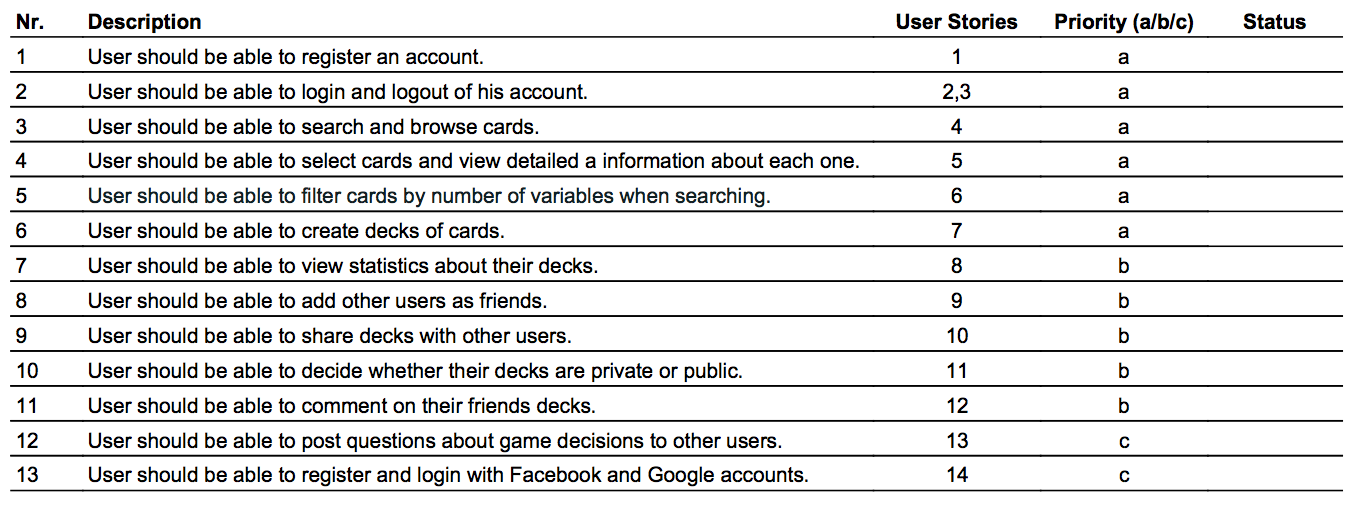
\includegraphics[width=1\textwidth]{RequirementList.png}}
\end{center}
\subsection{Non-functional Requirements}
\begin{center}
  \makebox[\textwidth]{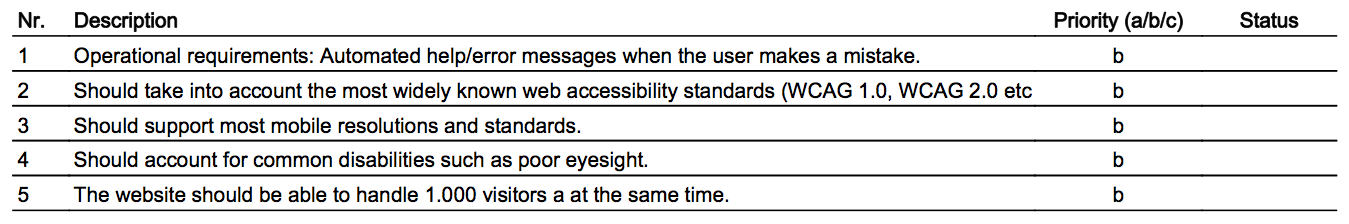
\includegraphics[width=1\textwidth]{non-functional.png}}
\end{center}

\section{User Stories}
The user stories describe the requirements in an everyday language. They also suggest a reason for wanting to be able to complete the tasks. They are meant to be simple and easy to understand and should make a good checklist when implementing the system. The user stories are ordered by priority, with the red boxes containing the highest priority stories, the yellow the intermediate ones and the green the lowest priority. Although the yellow and green user stories might not be implemented they are nevertheless included in case the organization of the project, or the priority of the user stories, changes in any way.
\begin{center}
  \makebox[\textwidth]{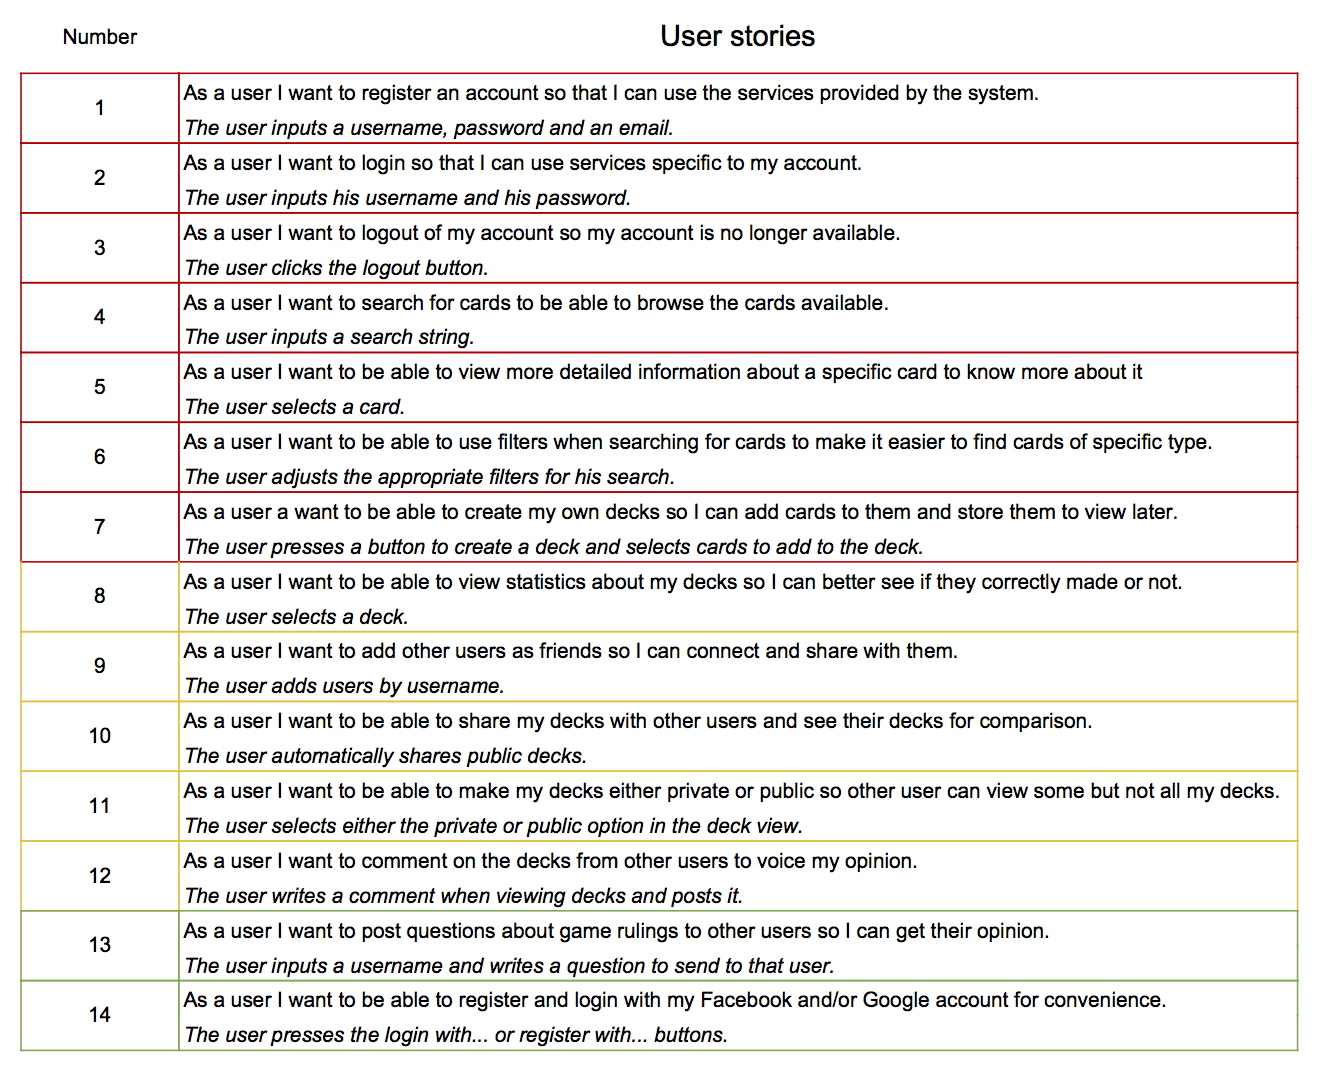
\includegraphics[width=1\textwidth]{UserStories.png}}
\end{center}

\section{Usability Goals}
I decided to set a few target goals for new users, if more than 80\% of them are able to perform the tasks with the given constraints then the system’s usability is satisfactory, but of course experienced users should easily be able to outperform the constraints.
\begin{itemize}
  \item The user should be able to register an account in under 2 minutes.
  \item The user should be able to login in less than 20 seconds.
  \item The user should be able to search for a card in less than a minute.
  \item The user should be able to create a deck in less than a minute.
  \item The user should be able to log out in less than 20 seconds.
  \item The user should be able to get to the homepage in one click from any page.
\end{itemize}

\section{Prototypes}
For the first draft layout of the website I made a few wireframes that give a good overview of the website. I also made some graphic design prototypes for reference but they do not necessarily portray the final look of the website since functionality will always be the highest priority.
\subsection{Wireframes}
The first wireframe describes the front page of the website. It has the same layout as all other pages on the site but if the user is not logged in he will be prompted with the register option in the top right corner of the page but the logout option otherwise.
\begin{center}
  \makebox[\textwidth]{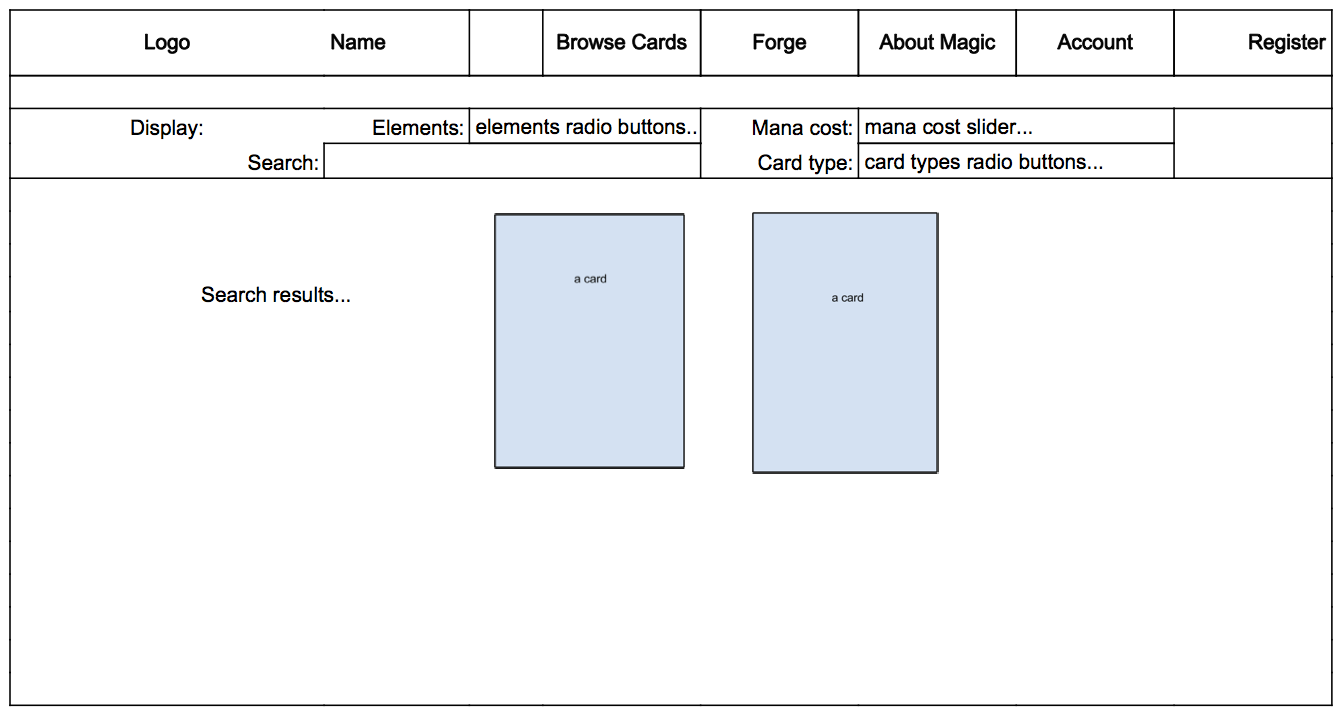
\includegraphics[width=1\textwidth]{WireframeFrontPage.png}}
\end{center}
The login page will also have the same layout as the other pages but display a login form where the user can insert his login information or press register if the user doesn’t have an account. The register page is the same as the login page except it displays a register form.
\begin{center}
  \makebox[\textwidth]{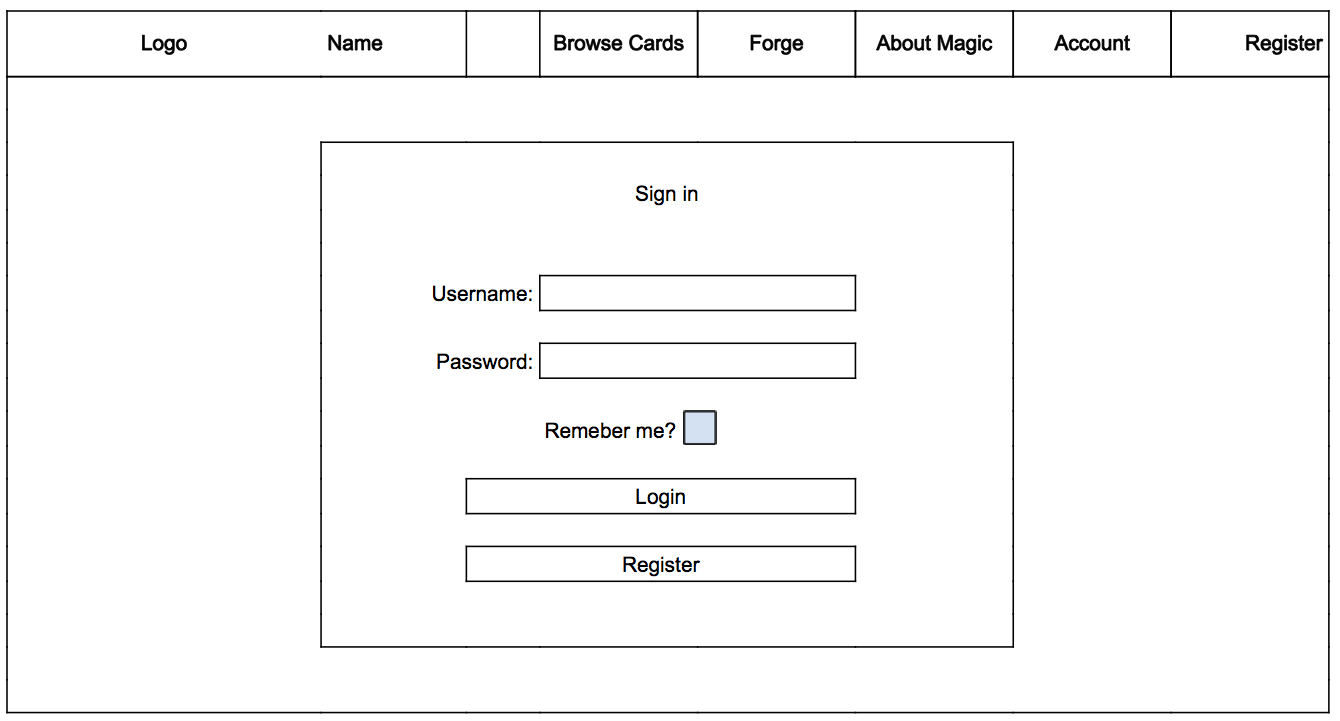
\includegraphics[width=1.1\textwidth]{WireframeSignIn.png}}
\end{center}
The forge is only available for logged in user. It has the same layout as other pages but displays the logout option in the top right corner. It gives the user the options to view their favorite cards, create new decks or navigate between already made decks and has the same search as the front page where the user can search for cards and add them to their decks. The current deck is then displayed below.
\begin{center}
  \makebox[\textwidth]{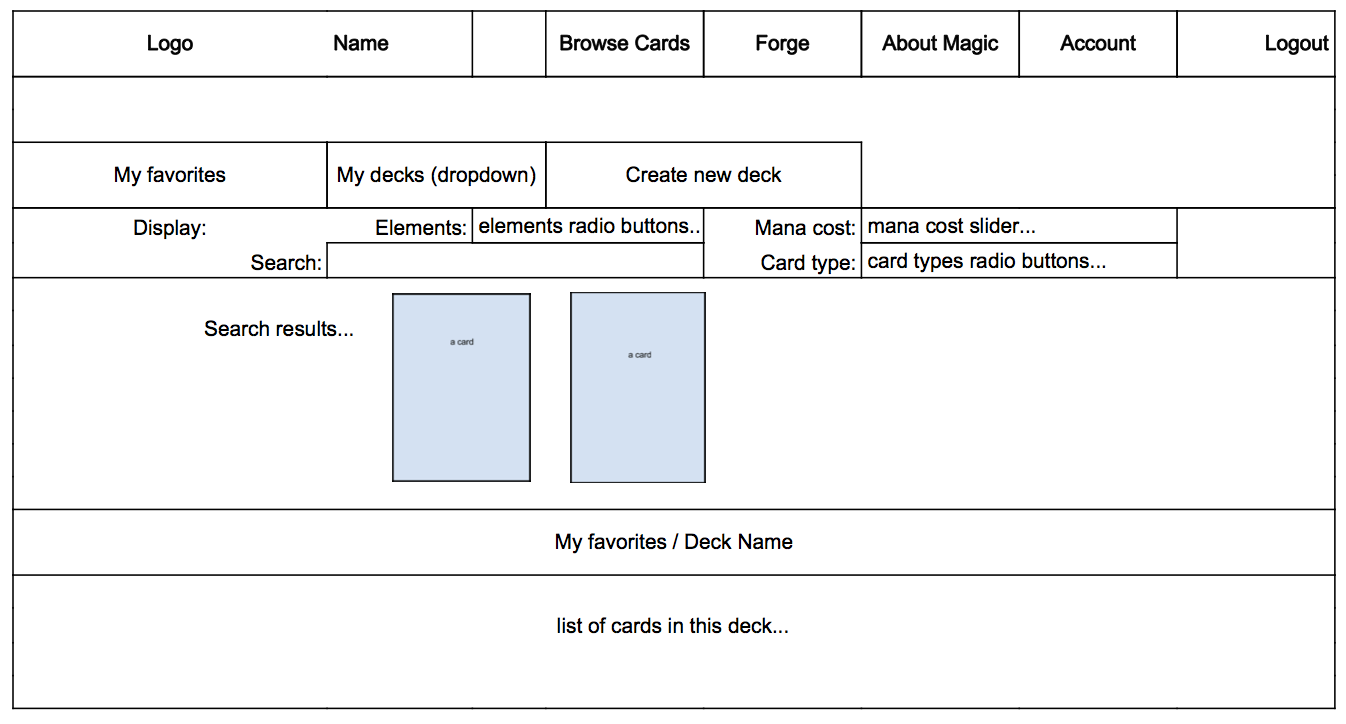
\includegraphics[width=1.1\textwidth]{forge.png}}
\end{center}
The about magic page will have the same layout as the others with either logout or register in the top right corner, depending on whether the user is logged in or not. The main area will then display a tab bar that a user can use to exchange the information displayed.
\begin{center}
  \makebox[\textwidth]{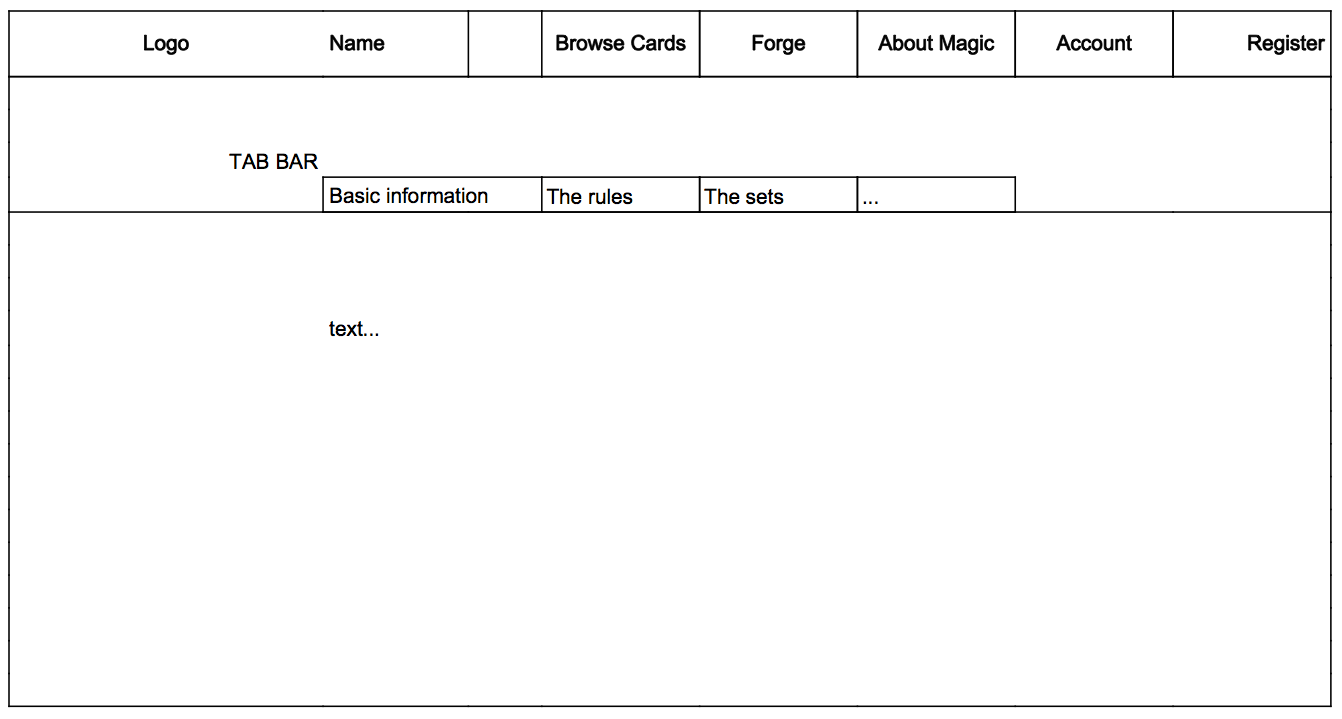
\includegraphics[width=1.1\textwidth]{aboutMagic.png}}
\end{center}

\subsection{Graphic Design}
These prototypes were mostly made as a reference and were only meant to portray the final design if time allows.
\begin{center}
  \makebox[\textwidth]{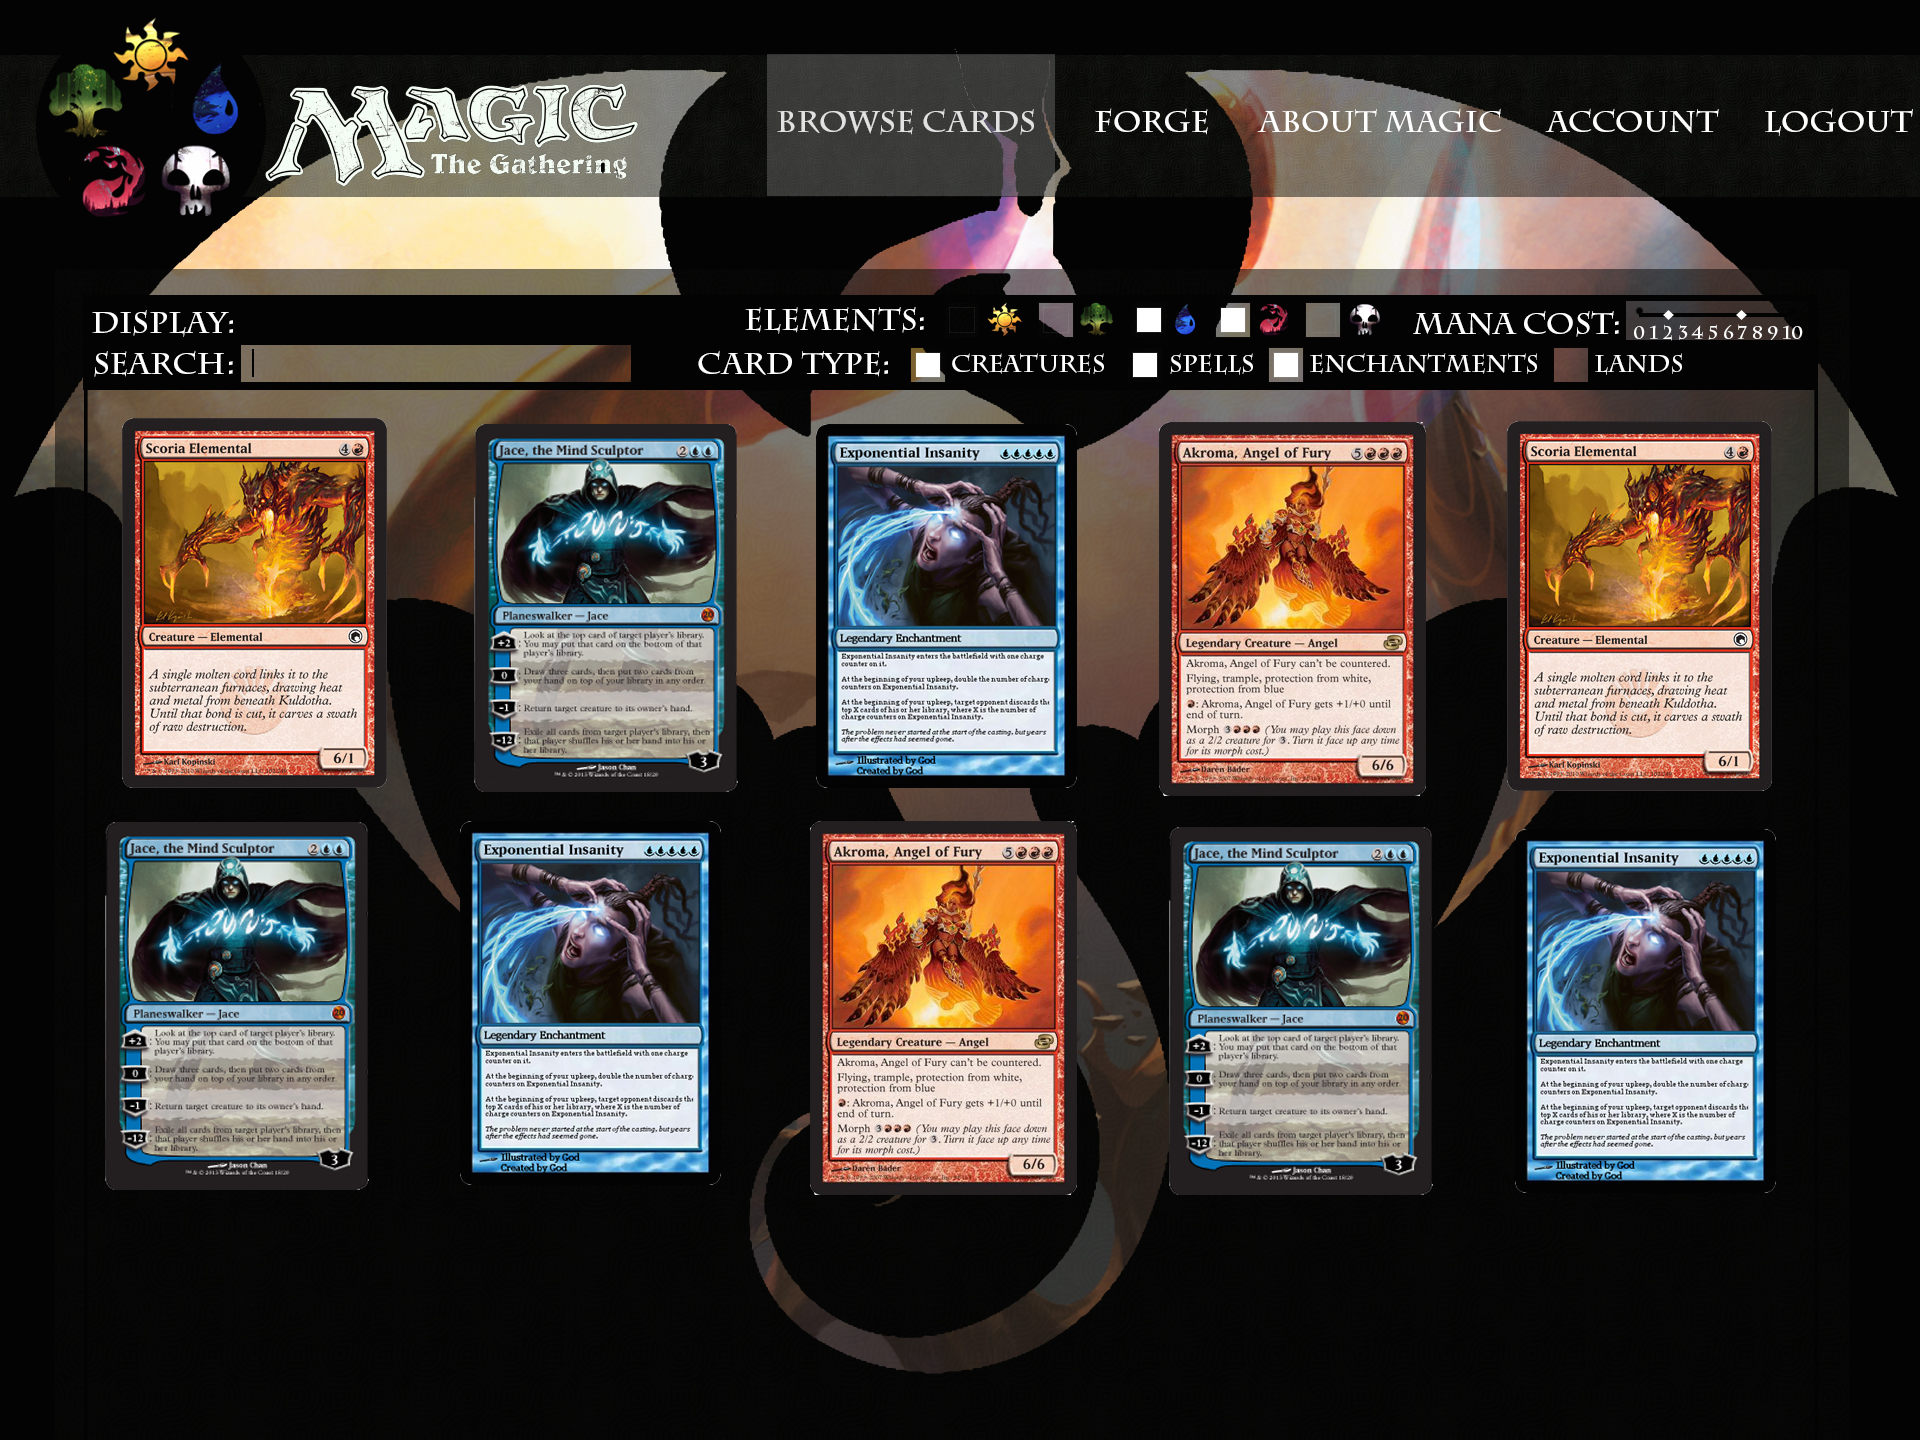
\includegraphics[width=0.8\textwidth]{FrontPage.png}}
\end{center}

\section{Navigation Diagram}
This diagram is meant as an overview of the navigation throughout the system. The diagram describes how the user navigates between pages and the two frames shows the difference in navigation when the user is logged in and when he is not.
\begin{center}
  \makebox[\textwidth]{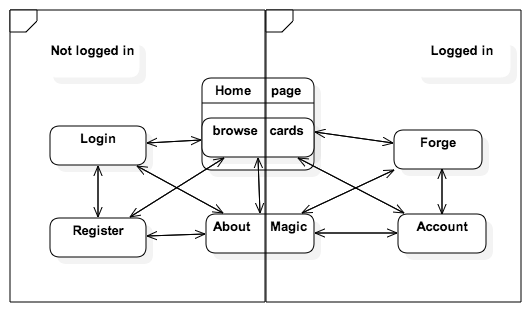
\includegraphics[width=0.5\textwidth]{StatechartDiagram1.png}}
\end{center}

\section{Class Diagram}
about the class diagram...
the diagram...
%   \subsection{Class Diagram}
% \begin{center}
%   \makebox[\textwidth]{\includegraphics[width=\paperwidth]{charts/ClassDiagram.png}}
% \end{center}

\section{The Database}
about the database development... 

\section{Description of Technical Environment}
During the programming phase I will explore different ways of developing the system. The following tools have been and will be used during preparation and production of the system.
\begin{itemize}
  \item All the code behind the system will be written in Visual Studio 2013 in the MVC5 environment.
  \item For assistance I will use Sublime Text 2 while coding.
  \item The system will be designed primarily with Google Chrome making use of the built in development tools.
  \item For javascript debugging I will use jslint.com as well as the development tools in Google Chrome.
  \item Source control will be provided with git.
  \item For source control hosting, I will use github.com, and connect to github through the team explorer in Visual Studio.
  \item I will use bootstrap to make visualisation changes to the website, but also to ensure accessibility and responsiveness of the website.
  \item The prototypes are implemented in Google Spreadsheet and Photoshop.
  \item The navigation diagram and class diagram were made in StarUML.
  \item Google Docs and \LaTeX \enspace was used to make the reports.
\end{itemize}

\section{Programming Rules}
I decided to put forth a few programming rules to follow, for better consistency and readability of code. First I looked at the XHTML standard for HTML and some CSS coding standards. I looked into Microsoft traditions for C\# and explored common traditions for JavaScript code. I adjusted the rules for my purposes and they are listed below with a few examples for clarity.
  \subsection{\textsc{html}}
  \begin{itemize}
    \item All attributes, events, and tags must be written in lower case.
    \item All elements must be closed.
    \item The value assigned to an attribute must be enclosed in quotes.
    \item All elements must be properly nested.
    \item Attribute minimization is not allowed (selected must be selected=`selected').
    \item Comment the code.
    \item Declare the correct doctype.
    \item Never use inline styles.
    \item Place external CSS files within the head \& put  javascript files at the bottom.
    \item Never use inline javascript.
    \item Use h1 - h6 tags properly.
    \item Use labels for all form boxes.
    \item Use unordered list for navigation.
    \item Always place the alt attribute for images.
  \end{itemize}
  \lstinputlisting[language=HTML]{ProgrammingRules/HTMLrules.html}

  \subsection{CSS}
  \begin{itemize}
    \item When grouping selectors, keep individual selectors to a single line.
    \item Use classes in selectors but avoid id's for better reusability of code.
    \item Include one space before the opening brace of declaration blocks for legibility.
    \item Place closing braces of declaration blocks on a new line.
    \item Selectors names should start with a lowercase letter.
    \item Id names should have underscores: \#user\_image.
    \item Class names should have hyphens: .profile-image.
    \item Only use English words.
    \item Group related items together with comments.
    \item Class and id names should be descriptive.
    \item CSS files should be organized using flags.
    \item Avoid shorthand CSS.
    \item All CSS should be in an external stylesheet, no inline styles.
    \item HTML first then CSS.
    \item Comment the CSS code.
    \item Use bootstrap whenever possible.
    \item Avoid extra selectors.
  \end{itemize}
  \lstinputlisting{ProgrammingRules/CSSrules.css}
  \subsection{C\#}
  \begin{itemize}
    \item Only use English words.
    \item When code is being indented, the `tab' button should be used (in Visual Studio 2013 `tab' is saved as four spaces).
    \item Use predefined type names instead of system type names like Int32, String, Single, UInt64, etc.
    \item Use camelCasing for method arguments and local variables.
    \item Use PascalCasing for class names and method names.
    \item Use noun or noun phrases to name a class.
    \item Vertically align curly brackets.
    \item Declare all member variables at the top of a class, with static variables at the very top.
    \item Commenting Conventions:
    \begin{itemize}
    \item Place the comment on a separate line, not at the end of a line of code.
    \item Begin comment text with an uppercase letter.
    \item End comment text with a period.
    \item Should be written in English.
    \end{itemize}
    \item Always specify [HttpPost] or [HttpGet].
    \item Use a try-catch statement for most exception handling.
    \item Avoid using abbreviations in names.
    \item Do not use underscores in identifiers.
    \item Singular names for enums.
    \item Do not use the word enum in enum names.
    \item Do not push code that doesn’t compile!
    \item Avoid complex expressions.
    \item Consider warnings as errors.
    \item Set a region around code that is related to one another.
    \item Use implicitly typed local variables when the variable type is clear.
    \item Use explicitly typed local variables when the variable type is not clear.
  \end{itemize}
  \lstinputlisting{ProgrammingRules/csrules.cs}
  \subsection{JavaScript}
  \begin{itemize}
    \item In general, use camelCasing for functions, variables and methods. Use PascalCasing for classes and enums. Constant values should be in all caps.
    \item Always use semicolons.
    \item Always use ‘var’ while declaring variables.
    \item Vertically align curly brackets.
    \item Declare variables outside of the ‘for’ statement.
    \item Never pass a string to SetInterval and SetTimeOut. Instead, pass a function name.
    \item Javascript files should be stored in an external file (not inline).
    \item The code should be correctly indented.
    \item Line length should not exceed 80 characters.
    \item Variables should be declared before they are used.
    \item Use === and !== in comparisons instead of == and !=.
    \item Comment your code.
    \end{itemize}
  \lstinputlisting{ProgrammingRules/javascriptrules.js}

\section{The Production Process}
\subsection{How the overall production fared}
\subsection{What went wrong and how it can be done better next time
}

\section{Requirements Outcome}
\subsection{What Requirements were met}
\subsection{What Requirements where left out and why}
\subsection{What Requirements where not finished and why}

\section{Usability Goals Outcome}

\section{Changes from Initial Analysis and Design}
\subsection{Interface Design}
\subsection{Class Diagram}

\section{Word Definitions}
\begin{itemize}
\item ...
\end{itemize}

\clearpage

\section{References}

\end{document}
